\documentclass[tikz,border=0pt]{standalone}

\usetikzlibrary{positioning}

\begin{document}

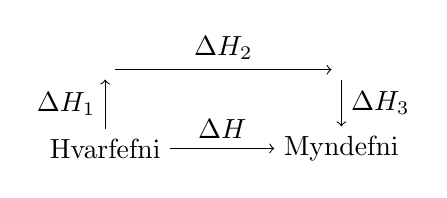
\begin{tikzpicture}[node distance=2cm]

% nodes
\node (A) at (0, 0) {Hvarfefni};
\node (B) at (0, 1) {};
\node (C) at (3, 1) {};
\node (D) at (3, 0) {Myndefni};

% arrows
\draw [->] (A) to node [left]{$\Delta H_1$} (B);
\draw [->] (B) to node [above]{$\Delta H_2$} (C);
\draw [->] (C) to node [right]{$\Delta H_3$} (D);

\draw [->] (A) to node [above]{$\Delta H$} (D);


\end{tikzpicture}

\end{document}

  
